
        \documentclass[spanish, 11pt]{exam}

        %These tell TeX which packages to use.
        \usepackage{array,epsfig}
        \usepackage{amsmath, textcomp}
        \usepackage{amsfonts}
        \usepackage{amssymb}
        \usepackage{amsxtra}
        \usepackage{amsthm}
        \usepackage{mathrsfs}
        \usepackage{color}
        \usepackage{multicol, xparse}
        \usepackage{verbatim}


        \usepackage[utf8]{inputenc}
        \usepackage[spanish]{babel}
        \usepackage{eurosym}

        \usepackage{graphicx}
        \graphicspath{{../img/}}
        \usepackage{pgf}



        \printanswers
        \nopointsinmargin
        \pointformat{}

        %Pagination stuff.
        %\setlength{\topmargin}{-.3 in}
        %\setlength{\oddsidemargin}{0in}
        %\setlength{\evensidemargin}{0in}
        %\setlength{\textheight}{9.in}
        %\setlength{\textwidth}{6.5in}
        %\pagestyle{empty}

        \let\multicolmulticols\multicols
        \let\endmulticolmulticols\endmulticols
        \RenewDocumentEnvironment{multicols}{mO{}}
         {%
          \ifnum#1=1
            #2%
          \else % More than 1 column
            \multicolmulticols{#1}[#2]
          \fi
         }
         {%
          \ifnum#1=1
          \else % More than 1 column
            \endmulticolmulticols
          \fi
         }
        \renewcommand{\solutiontitle}{\noindent\textbf{Sol:}\enspace}

        \newcommand{\samedir}{\mathbin{\!/\mkern-5mu/\!}}

        \newcommand{\class}{1º Bachillerato}
        \newcommand{\examdate}{\today}

        \newcommand{\tipo}{A}


        \newcommand{\timelimit}{50 minutos}



        \pagestyle{head}
        \firstpageheader{
\includegraphics[width=0.2\columnwidth]{header_left}}{\textbf{Departamento de Matemáticas\linebreak \class}\linebreak \examnum}{
\includegraphics[width=0.1\columnwidth]{header_right}}
        \runningheader{\class}{\examnum}{Página \thepage\ of \numpages}
        \runningheadrule

        \newcommand{\examnum}{Continuidad}
        \begin{document}
        \begin{questions}
        \question Ejercicios2:  - Calcula los siguientes límites:

        \begin{multicols}{3}
        \begin{parts} \part[1] $$\lim_{x \to -2}\left(\frac{2 x^{2} + 7 x + 6}{x^{3} + 3 x^{2} + 3 x + 2}\right)$$  \begin{solution}   $- \frac{1}{3}$   \end{solution} \part[1] $$\lim_{x \to -1}\left(\frac{x^{3} + 1}{x^{2} + 2 x + 1}\right)$$  \begin{solution}   No existe el límite   \end{solution} \part[1] $$\lim_{x \to \infty} \left(\frac{3 x - 1}{3 x - 2}\right)^{2 x}$$  \begin{solution}   $e^{\frac{2}{3}}$   \end{solution}
        \end{parts}
        \end{multicols}
        \question ejfunc1-0 - Dada la función:$f(x)=\frac{x^{2} - 2 x + 1}{2 x + 3}$, calcular:
        \begin{multicols}{1}
        \begin{parts} \part[1] Dominio de $f(x)$  \begin{solution}   $Dom(f)=\left(-\infty, - \frac{3}{2}\right) \cup \left(- \frac{3}{2}, \infty\right)$\\ \resizebox{0.4\textwidth}{!}{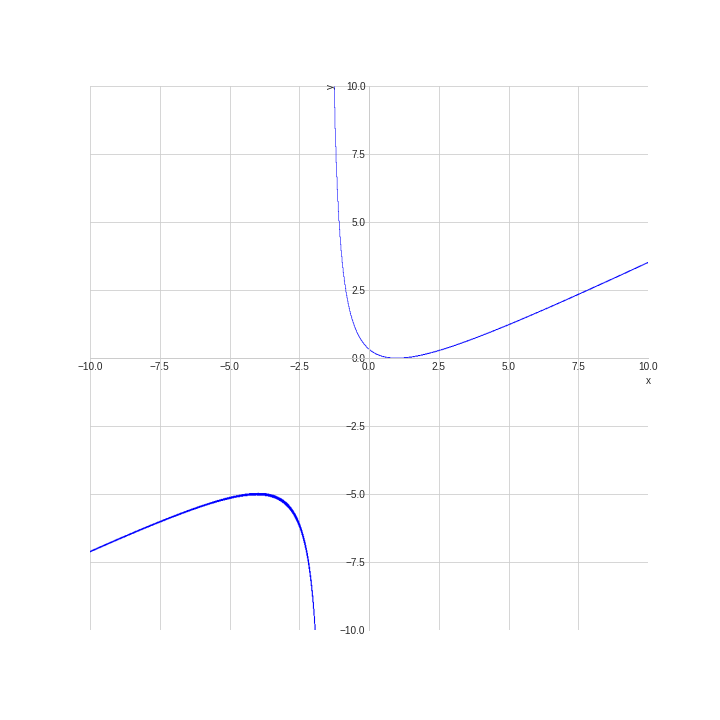
\includegraphics[width=1\columnwidth]{ejfunc1-0}}   \end{solution} \part[1] ¿Para qué valores de $x$ la función es creciente?  \begin{solution}   $\left(-\infty, -4\right) \cup \left(1, \infty\right)$   \end{solution} \part[1] Asíntotas verticales, horizontales y oblicuas, en caso que existan  \begin{solution}   Asíntotas:\\A.V. $x=-3/2$\\A.O. $y=\frac{x}{2} - \frac{7}{4}$ \\A.O. $y=\frac{x}{2} - \frac{7}{4}$ \\   \end{solution}
        \end{parts}
        \end{multicols}
        \question ejfunc1-1 - Dada la función:$f(x)=\frac{- x^{2} - x + 3}{x^{2} + x - 2}$, calcular:
        \begin{multicols}{1}
        \begin{parts} \part[1] Dominio de $f(x)$  \begin{solution}   $Dom(f)=\left(-\infty, -2\right) \cup \left(-2, 1\right) \cup \left(1, \infty\right)$\\ \resizebox{0.4\textwidth}{!}{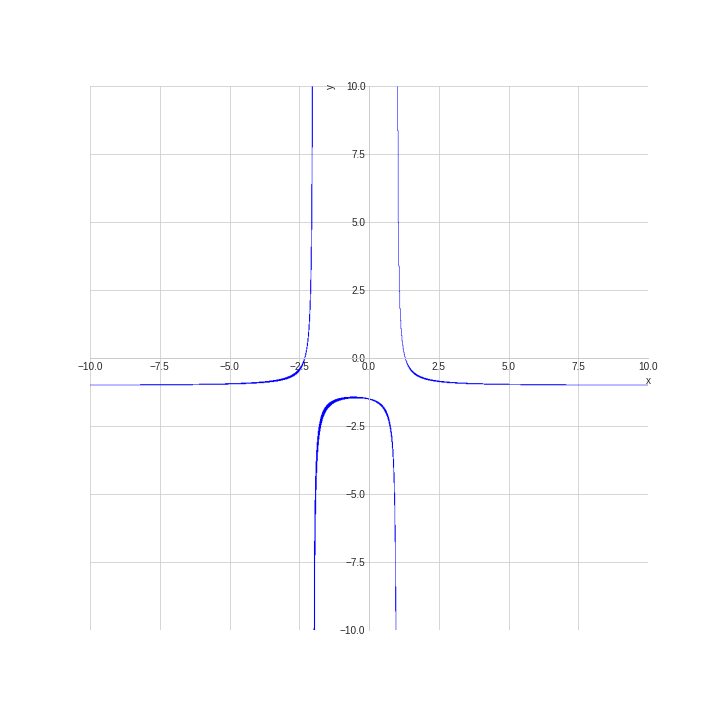
\includegraphics[width=1\columnwidth]{ejfunc1-1}}   \end{solution} \part[1] ¿Para qué valores de $x$ la función es creciente?  \begin{solution}   $\left(-\infty, -2\right) \cup \left(-2, - \frac{1}{2}\right)$   \end{solution} \part[1] Asíntotas verticales, horizontales y oblicuas, en caso que existan  \begin{solution}   Asíntotas:\\A.V. $x=-2$\\, A.V. $x=1$\\A.H. $y=-1$\\A.H. $y=-1$\\A.O. $y=-1$ \\A.O. $y=-1$ \\   \end{solution}
        
        \end{parts}
        \end{multicols}
        
    \end{questions}
    \end{document}
    